\selectlanguage{italian}

Il nucleo atomico è un sistema particolarmente complicato da descrivere, essendo un sistema a molti corpi quantistico legato dall'interazione forte, la quale non ha un'espressione ben definita come la forza coulombiana (non essendo neanche una forza che agisce a coppie di particelle).\\
In particolare, è possibile dare una duplice descrizione del nucleo, tenendo conto di diverse osservazioni sperimentali: da un lato è possibile vede il nucleo come un insieme di particelle singole, esprimendo gli stati nucleari in funzione delle singole eccitazioni dei vari nucleoni; dall'altro è invece possibile descrivere il nucleo come una sorta di $ \virgolette{liquid drop} $ (riprendendo il modello di Weiszäcker), così da poter tener conto dei moti collettivi nucleari che si osservano.

\section{Nuclear shell model}

La descrizione del nucleo come insieme di particelle singole porta ad un modello analogo al modello atomico a shell, sotto l'ipotesi che i nucleoni si muovano indipendentemente gli uni dagli altri in un potenziale a simmetria sferica: questo però è vero solo nell'intorno di determinati valori di $ Z $ e $ N $, mentre in realtà la maggior parte dei nuclei sono deformati.

\subsection{Atomic physics}

Il modello atomico a shell descrive gli elettroni dell'atomo come disposti su una serie di livelli energetici, detti shells, posti a determinate distanza (sia spaziali che energetiche) tra loro.\\
In particolare, gli elettroni sono descritti da quattro quantum numbers $ \ket{n,\ell,m,s} $: quello principale $ n \in \N $, quello orbitale $ \ell \in [0,n-1] $, quello magnetico $ m \in [-\ell,\ell] $ e quello di spin $ s = \pm \frac{1}{2} $.\\
Nell'atomo più semplice, ovvero l'atomo di idrogeno $ \ch{^1H} $, si ha una degenerazione delle shells a diverso momento angolare:
\begin{equation}
	E_{n,\ell} = \alpha^2 \frac{m_e c^2}{2 (n + \ell)^2}
	\label{eq:5.1}
\end{equation}
dove $ \alpha = \frac{e^2}{4\pi \epsilon_0 \hbar c} $ è la costante di struttura fine. In presenza di deviazioni dal potenziale puro $ \sim \frac{1}{r} $ questa degenerazione viene rimossa: ciò avviene considerando la presenza di altri elettroni, che modificano il potenziale, e l'interazione spin-orbita, che porta al cosiddetto splitting fine.\\
Il modello atomico a shell può essere giustificato sia a livello teorico che sperimentale. Innanzitutto il potenziale può essere assunto come quello Coulombiano a simmetria sferica poiché $ R_{\text{nucleo}} \ll R_{\text{atomo}} $, ed inoltre il centro del potenziale è ben definito poiché $ M_{\text{nucleo}} \gg M_{\text{elettroni}} $: una volta determinato in questo modo il potenziale, tutto deriva dalle leggi di quantizzazione del momento angolare e dal principio d'esclusione di Pauli. A livello sperimentale, invece, esso può essere confermato studiando l'andamento di varie proprietà atomiche; ad esempio, in Fig. \ref{atom-prop} sono riportati il raggio atomico e l'energia di prima ionizzazione dei vari atomi: si può notare che, in corrispondenza delle varie shell closures, si evidenziano notevoli discontinuità nell'andamento altrimenti piuttosto monotono di tali quantità. Le shell closures altro non sono che il completo riempimento delle varie subshells magnetiche di ciascuna shell a dato momento angolare: infatti, una shell associata ad un determinato $ \ell $ ha $ 2\ell + 1 $ subshells degeneri a causa di $ m $, con un ulteriore fattore $ 2 $ dovuto ad $ s $; dunque, fissato il livello energetico $ n $, il numero di elettroni che possono occupare tale livello è:
\begin{equation}
	Z_n = \sum_{\ell = 0}^{n - 1} 2(2\ell + 1) = 2n^2
	\label{eq:5.2}
\end{equation}
Ordinando gli orbitali $ n\ell $ in base alla loro energia e seguendo la \textit{regola dell'Aufbau} (o regola $ n + \ell $), si trovano le shell closures in corrispondenza di $ Z = 2,10,18,36,\dots $, ovvero quelli che nel sistema periodico vengono chiamati elementi nobili: questi sono caratterizzati da un momento angolare totale nullo $ J = 0 $, un'elevata energia di legame ed una bassa reattività.

\begin{figure}[!t]
	\centering
	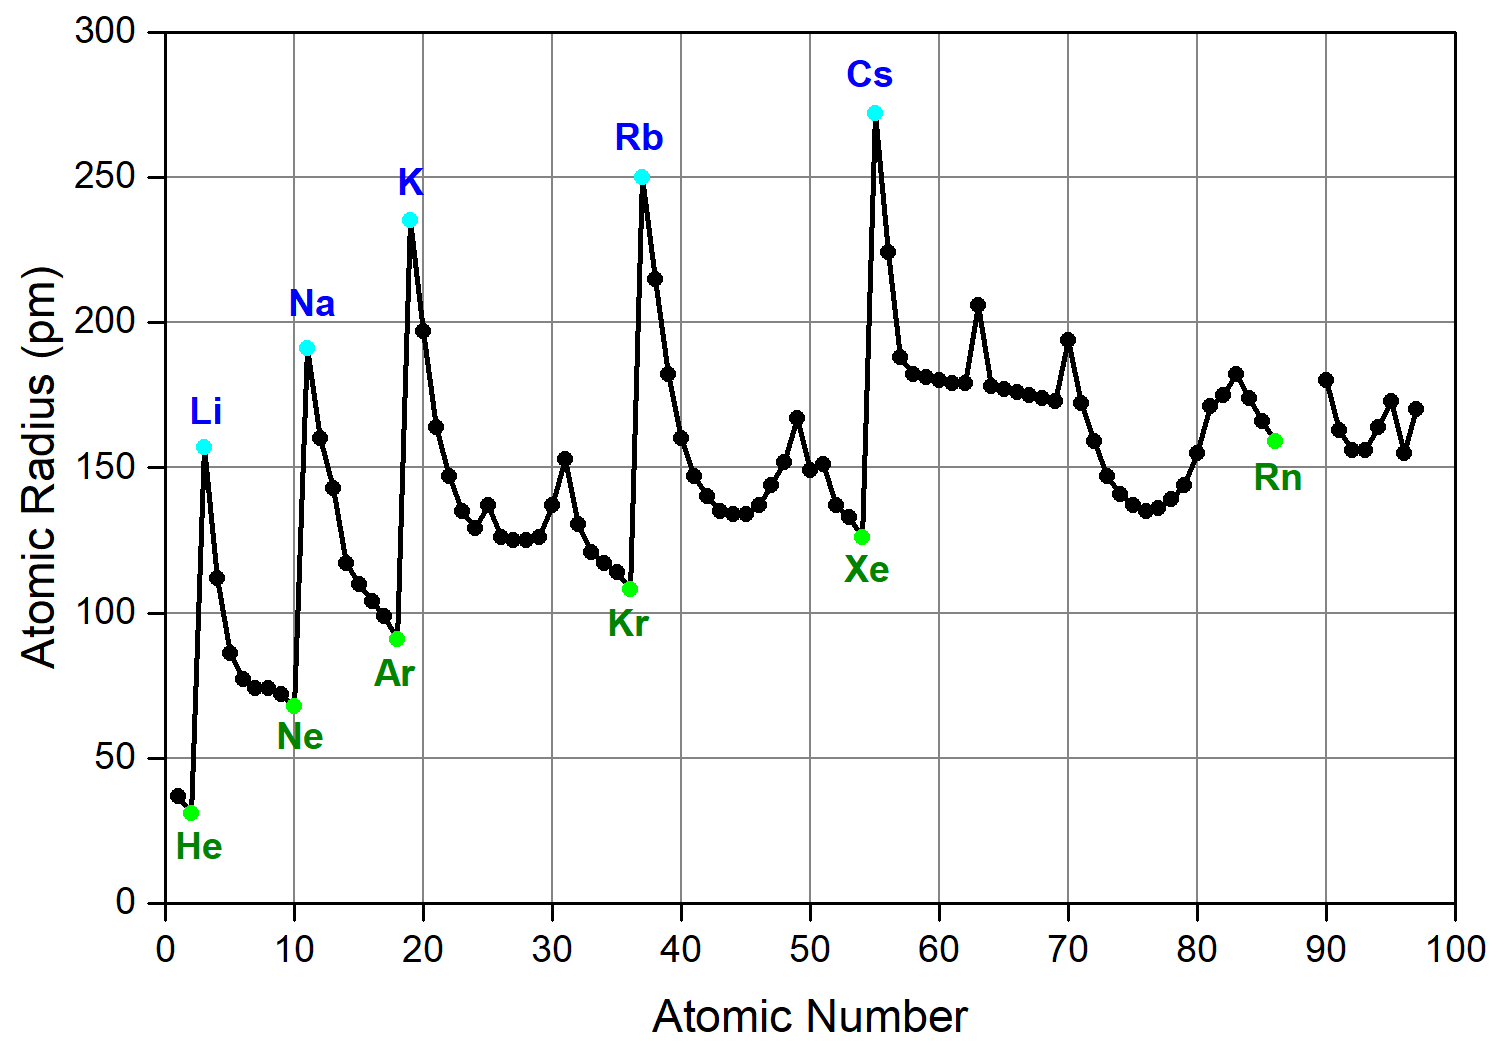
\includegraphics[width=0.45\textwidth]{atom-rad.png}
	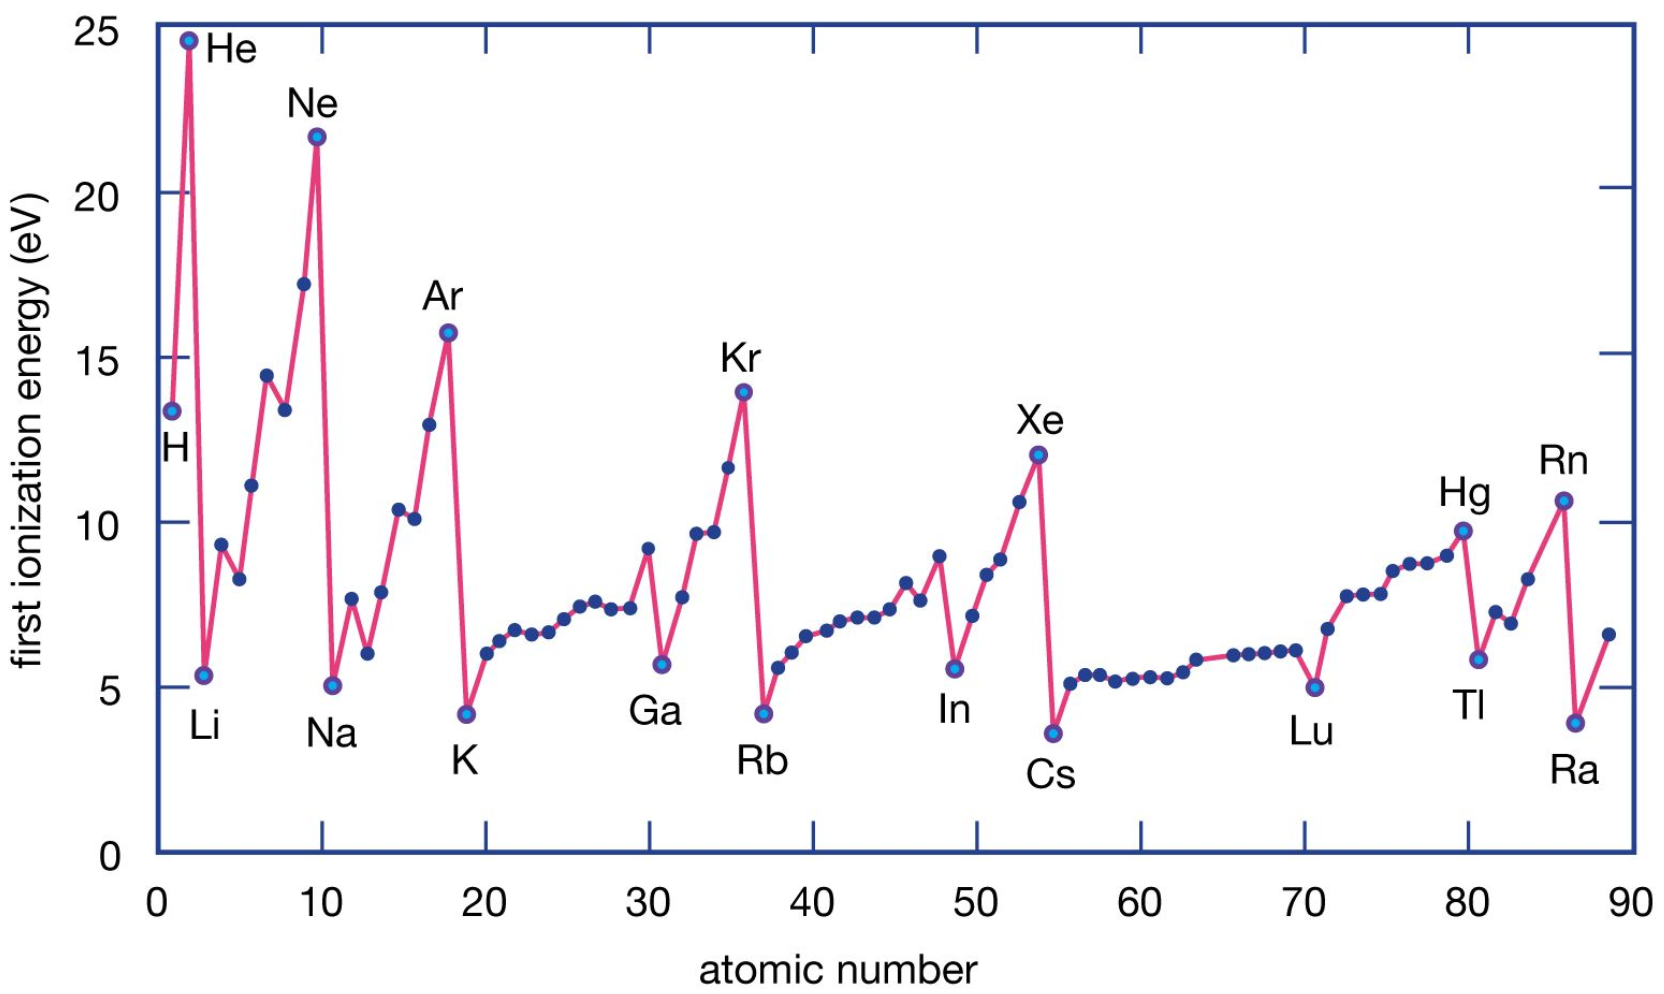
\includegraphics[width=0.52\textwidth]{atomic-ion-en.png}
	\caption{Atomic radius and ionization energy as functions of atomic mass number.}
	\label{atom-prop}
\end{figure}

\subsection{Evidenze sperimentali}

La semplicità del modello atomico a shell non è così immediata da traslare alla fisica nucleare: infatti, mentre gli elettroni nell'atomo sono soggette al campo coulombiano generato dal nucleo atomico, nel nucleo i nucleoni sono soggetti ad un campo che essi stessi generano, rendendo la trattazione analitica estremamente più complicata; inoltre, i nucleoni hanno un raggio relativamente grande rispetto al raggio del nucleo, a differenza degli elettroni che possono essere approssimati come point particles all'interno dell'atomo: ciò rende il concetto di orbite spaziali ben definite difficile da applicare al nucleo, dove il moto dei nucleoni può essere disturbato da urti con altri nucleoni.\\
Nonostante ciò, ci sono varie evidenze sperimentali che suggeriscono l'esistenza di shell nucleari.\\
Innanzitutto, se si plotta la binding energy per nucleone (Fig. \ref{magic-bind-en}), si notano delle consistenti deviazioni dalla formula di Weizsäcker per il liquid drop model in corrispodenza di precisi valori (uguali) di $ N $ e $ Z $, detti magic numbers: 2, 8, 20, 28, 50, 82, 126. Ciò significa che i nuclidi con determinati numeri di neutroni e/o protoni sono più legati, e dunque più stabili, dei nuclidi ad essi adiacenti. Per completezza, si ricordi che il liquid drop model non si applica per $ A < 20 $, poiché tali nuclidi presentano una struttura nucleare più complessa.

\begin{figure}[!t]
	\centering
	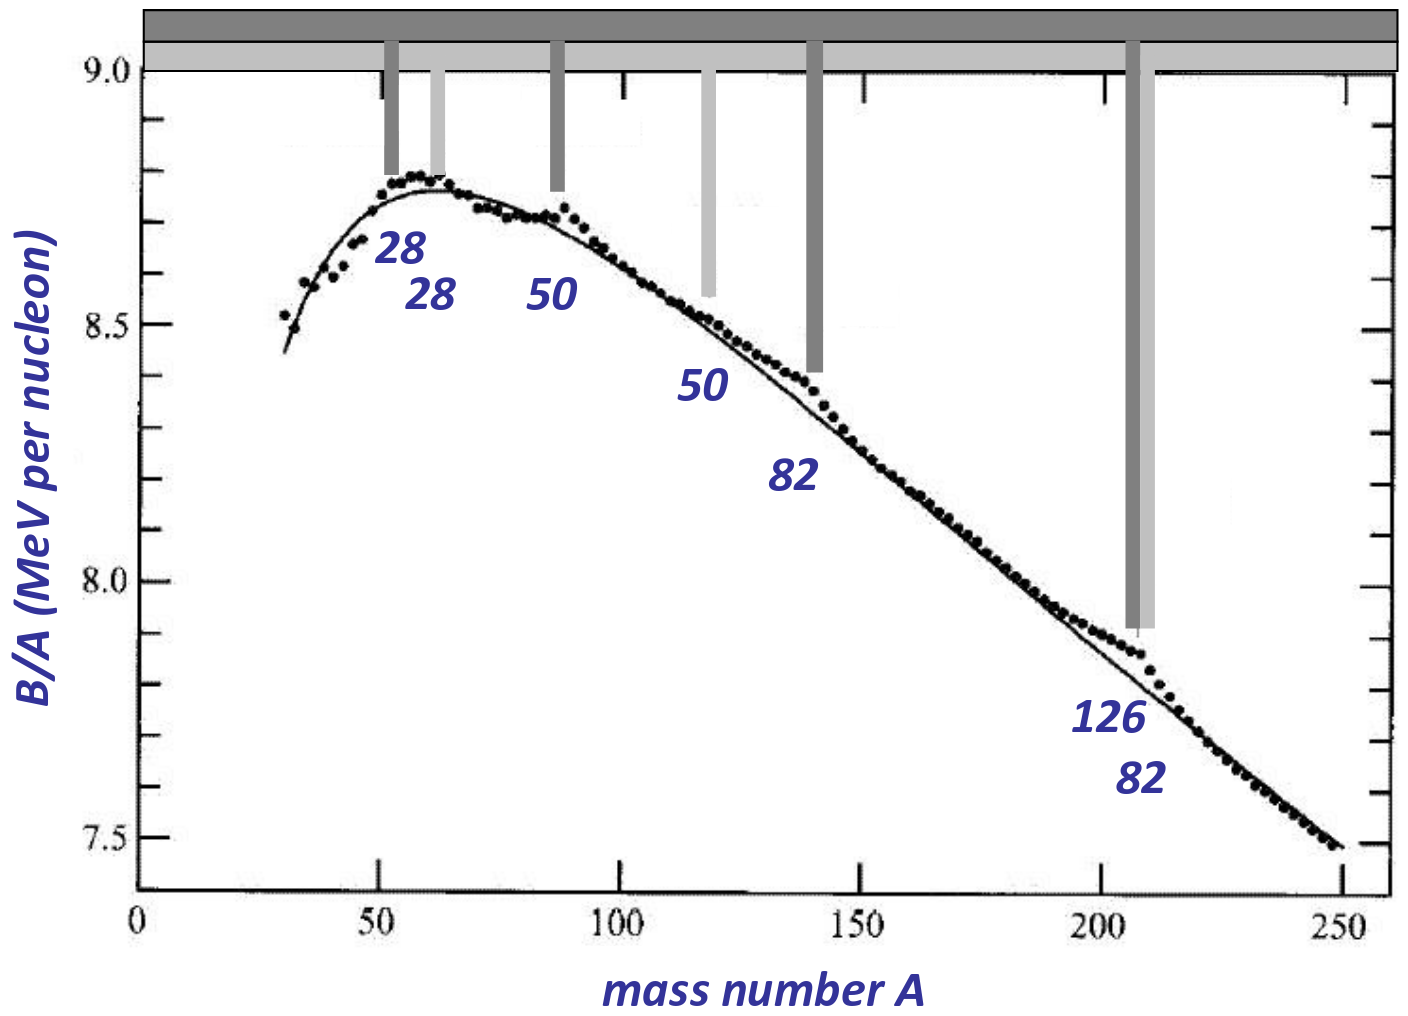
\includegraphics[width=0.60\textwidth]{magic-bind-en.png}
	\caption{Binding energy per nucleon, with $ N $ (dark grey) and $ Z $ (light grey) highlighted.}
	\label{magic-bind-en}
\end{figure}

\begin{figure}[!ht]
	\centering
	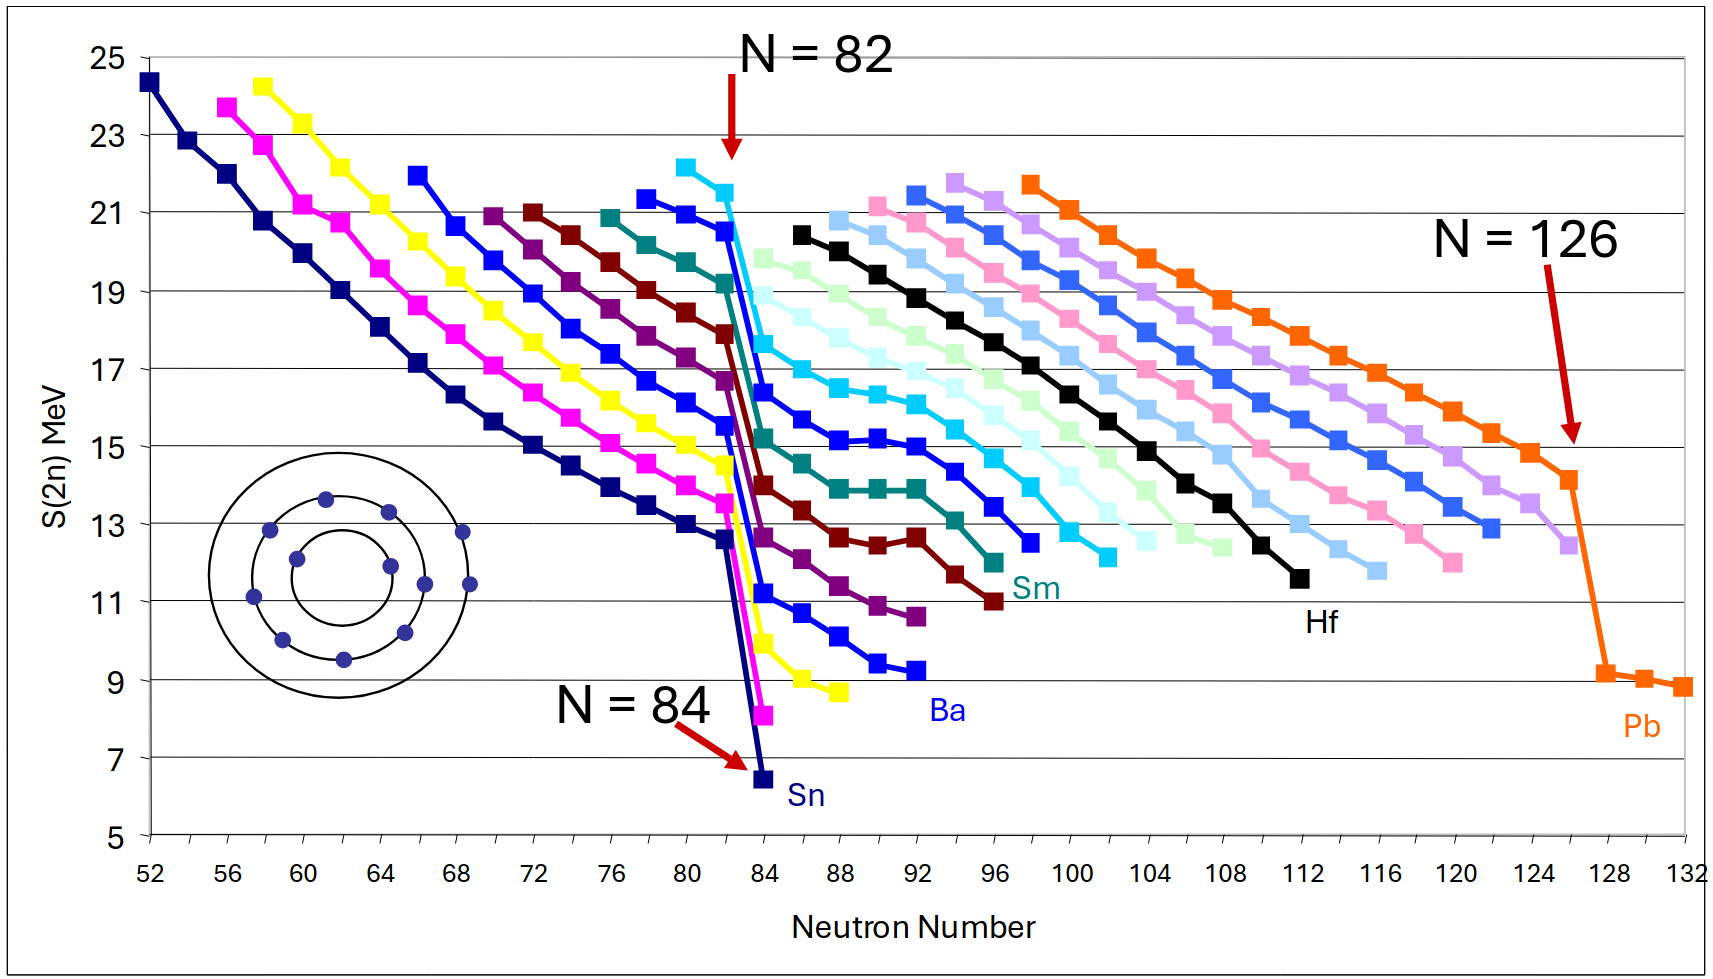
\includegraphics[width=0.60\textwidth]{2-n-b-e.png}
	\caption{2-neutron binding energy as a function of $ N $ for various isotopic chains.}
	\label{2-n-b-e}
\end{figure}

\begin{figure}[!t]
	\centering
	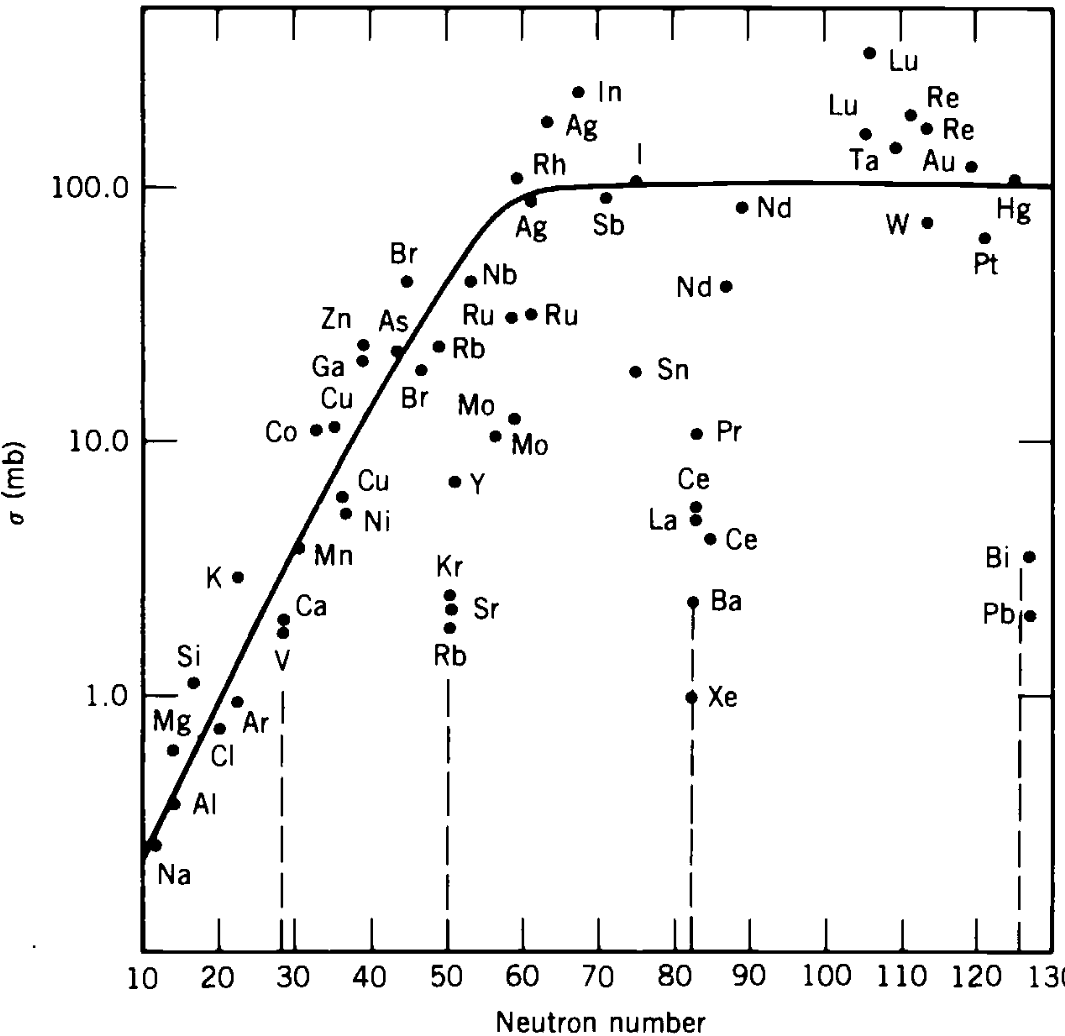
\includegraphics[width=0.60\textwidth]{magic-n-cap.png}
	\caption{$ n $-capture cross-section ad a funzion of.}
	\label{n-cap-cr}
\end{figure}

Gli stessi magic numbers si notano studiando la cosiddetta \textit{2-neutron binding energy}, ovvero la quantità $ S_{2n}(N,Z) \equiv B(N,Z) - B(N-2,Z) $, come si può vedere in Fig. \ref{2-n-b-e}: ciò può essere interpretato come una maggiore stabilità data dal completamento di shell neutroniche.\\
Anche l'abbondanza di isotopi stabili nel sistema solare mostra dei picchi in corrispondenza dei magic numbers, evidenziando la particolare stabilità dei nuclidi con shell closures.\\
Inoltre, la cross-section per la cattura neutronica subisce delle riduzioni di un paio di ordini di grandezza in corrispondenza dei magic numbers (Fig. \ref{n-cap-cr}: ciò è sia conseguenza diretta delle shell closures, sia conseguenza della riduzione del raggio nucleare determinato dalle suddette (dato che $ \sigma \sim \pi R^2 $).
Infine, per nuclei vicini ai magic numbers si osservano degli stati eccitati relativamente long-lived ($ \tau > 10^{-6}\,\text{s} $) detti \textit{isomeri}: i magic numbers determinano delle cosiddette $ \virgolette{islands of isomerism} $.\\
Si deve aggiungere poi che il liquid drop model non consente una descrizione di vari proprietà nucleari come lo spin, la parità, i momenti magnetici etc. Inoltre, esso non predice la densità nucleare e tutti i suoi coefficienti sono puramente empirici.

\subsection{Modello a particelle indipendenti}

Il primo modello a shell in grado di riprodurre i magic numbers e le proprietà dei magic nuclei fu formulato nel 1949 da Mayer e Jensen (entrambi Nobel nel 1963).\\
Il cosiddetto extreme single-particle shell model, detto anche shell model a particelle indipendenti, ha come assunzione di base che i nucleoni possano muoversi nel nucleo per la maggior parte del tempo senza interagire con altri nucleoni: ciò equivale a dire che il libero cammino medio di un nucleone è maggiore delle dimensioni del nucleo. Ovviamente questa è solo una semplificazione, dato che l'interazione tra nucleoni ha effetti importanti.\\
Rispetto allo shell model atomico, quello nucleare deve tener conto di alcune complicazioni: innanzitutto la forma del potenziale non è nota e, qualora lo si volesse assumere centrale, non ha avrebbe un centro definito poiché ciascun nucleone è sorgente del campo; inoltre, i nucleoni occupano il  nucleo in modo continuo, dunque non è ovvio come estendere il concetto di orbitale in questo contesto. Quest'ultima difficoltà è in parte ridotta dal principio d'esclusione di Pauli e dal modello a gas di Fermi\footnote{Un gas di Fermi è un modello ideale di un ensamble di molti fermioni non-interagenti in equilibrio termico, descritto dalla statistica di Fermi-Dirac.}: se il gas di nucleoni è fortemente degenere, ciascun nucleone è in uno stato quantistico e non scattera con un altro nucleone se non con un meccanismo di scambio, il che permette di impostare un'equazione del moto per il singolo nucleone (da qui il nome di modello a particelle indipendenti).\\
Per rendere l'equazione di Schrödinger risolvibile per un singolo nucleone, si applica l'\textit{approssimazione di campo medio}:
\begin{equation*}
	\hat{\mathcal{H}} = \sum_{j = 1}^{A} \frac{\hat{p}_j^2}{2m_j} + \sum_{j \neq k}^{A} \hat{V}_k(r_j) = \sum_{j = 1}^{A} \left[ \frac{\hat{p}_j^2}{2m_j} + \hat{V}(r_j) \right] + \sum_{j = 1}^{A} \underbrace{\left[ \sum_{k \neq j}^{A} \hat{V}_k(r_j) - \hat{V}(r_j) \right]}_{0}
\end{equation*}
dove l'approssimazione consiste nell'ultima semplificazione. Ciò permette di sostituire il termine d'interazione (che è a 2 corpi solo in prima approssimazione) con un potenziale centrale medio, ignorando l'interazione residua. Dato che il potenziale ha simmetria sferica, è possibile separare la funzione d'onda come:
\begin{equation}
	\psi(\ve{r}) = \frac{u_{\ell}}{r} Y_{\ell,m}(\theta,\phi) X_s
	\label{eq:5.3}
\end{equation}
recuperando così gli ususali numeri quantici. Rimane da determinare il potenziale; i tre potenziali usuali sono quello coulombiano, la buca di potenziale e quello armonico: il potenziale coulombiano non è adatto poiché l'interazione nucleare è a breve raggio e poiché non può riprodurre la saturazione delle forze nucleari; la buca di potenziale non è realistica poiché non può riprodurre l'energia cinetica e potenziale dei nucleoni; il potenziale armonico non va a 0 all'infinito, dunque non potrebbe descrivere la fuoriuscita di nucleoni dal nucleo, cosa che avviene se ad esempio viene aggiunto un nucleone ad un nuclide debolmente legato. Il potenziale che meglio rappresenta l'interazione nucleare è il \textit{potenziale di Woods-Saxon}:
\begin{equation}
	V_{\text{WS}}(r) = \frac{-V_0}{1 + e^{(r - R_0) / a}}
	\label{eq:5.4}
\end{equation}
dove $ V_0 \approx 50\mev $ (verso le driplines varia drasticamente), $ R_0 \approx 1.25\fm \cdot A^{1/3} $ è il raggio nucleare medio e $ a \approx 0.524\fm $ è la skin thickness del nucleo (distanza in cui $ V(r) $ passa da $ 0.9 V_0 $ a $ 0.1 V_0 $); esso è plottato in Fig. \ref{woods-saxon}.

\begin{figure}[!b]
	\centering
	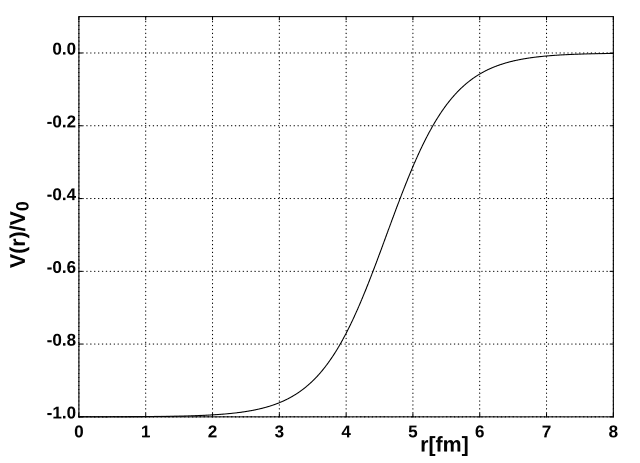
\includegraphics[width=0.70\textwidth]{woods-saxon.png}
	\caption{Woods-Saxon potential.}
	\label{woods-saxon}
\end{figure}

Il potenziale di Woods-Saxon prevede sia gli stati legati, con energia negativa, sia gli stati del continuo, con energia positiva. Gli stati sono giustamente quantizzati con tre numeri quantici: quello principale $ n $, quello angolare orbitale $ \ell $ e quello angolare totale $ j $ (relativo a $ \ve{J} = \ve{L} + \ve{S} $). Gli orbitali nucleari vengono quindi identificati come $ n\ell_j $, dove $ \ell $ è indicato con una lettera: $ s $ per $ \ell = 0 $, $ p $ per $ \ell = 1 $, $ d $ per $ \ell = 2 $, $ f $ per $ \ell = 3 $ e poi in ordine alfabetico.\\
Come si può vedere in Fig. \ref{ws-sp}, il solo potenziale di Woods-Saxon predice correttamente soltanto i primi tre magic numbers. È quindi necessario modificare tale potenziale con un termine di nuovo mutuato dalla fisica atomica: un termine d'interazione spin-orbita. Nel caso atomico, l'interazione spin-orbita avviene poiché il momento magnetico dell'elettrone interagisce col campo magnetico generato dal suo moto attorno al nucleo; nel caso nucleare, essa non deriva dall'interazione elettromagnetica ma dalla natura spin-dependent dell'interazione tra nucleoni.\\
Ricordando l'Eq. \ref{eq:4.20}, si può scrivere il \textit{potenziale d'interazione spin-orbita} come:
\begin{equation}
	V_{\ell,s}(r) \ve{L}\cdot\ve{S} = - \lambda \frac{1}{r} \frac{dV_{\text{WS}}}{dr} \ve{L}\cdot\ve{S}
	\label{eq:5.5}
\end{equation}
dove $ \lambda > 0 $ non ha particolare interesse fisico. Questo termine deriva dalla descrizione relativistica di un singolo nucleone nel nucleo ed è particolarmente importante sulla superficie nucleare (quando $ V_{\text{WS}}(r) $ varia maggiormente).

\begin{figure}[!b]
	\centering
	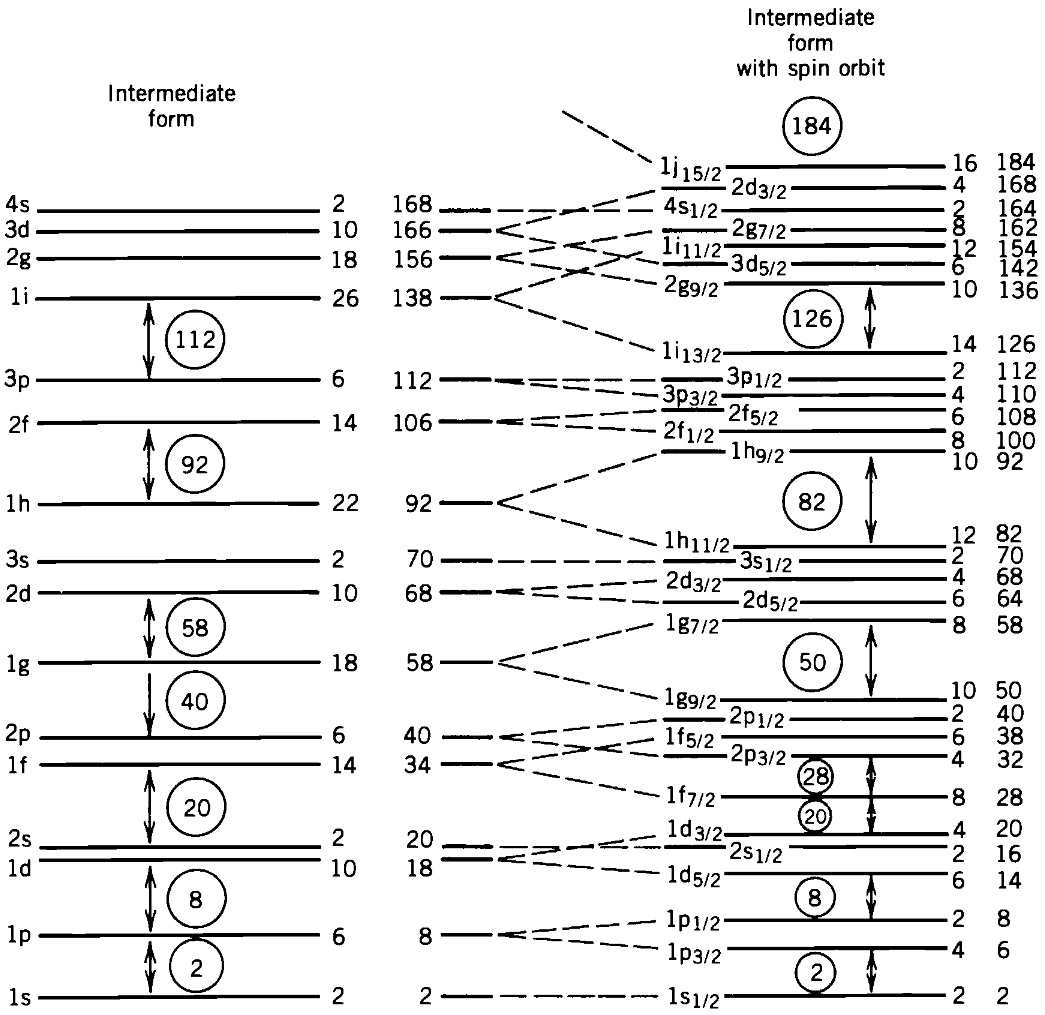
\includegraphics[width=0.60\textwidth]{ws-spectrum.png}
	\caption{Energy levels for the Woods-Saxon potential, without and with spin-orbit interaction.}
	\label{ws-sp}
\end{figure}

Si può vedere come l'aggiunta di questo termine splitti gli orbitali in modo da ottenere i corretti magic numbers. Ricordando che un nucleone ha $ s = \frac{1}{2} $, si vede che i possibili valori per $ j $ sono $ j = \ell + \frac{1}{2} $ e $ j = \ell - \frac{1}{2} $; inoltre, si può lavorare sul termine $ \ve{L}\cdot\ve{S} $:
\begin{equation*}
	\braket{\ve{L}\cdot\ve{S}} = \frac{1}{2} \braket{\ve{J}^2 - \ve{L}^2 - \ve{S}^2} = \frac{\hbar^2}{2} \left[ j (j + 1) - \ell (\ell + 1) - s (s + 1) \right]
\end{equation*}
A questo punto, si deve considerare che i due possibili valori di $ j $ per ogni $ \ell $ portano ad uno split degli orbitali considerati: ad esempio, un orbitale $ 1f $ (con $ \ell = 3 $) viene splittato in $ 1f_{5/2} $ e $ 1f_{7/2} $. Ciascun orbitale così ottenuto ha degenerazione $ 2j + 1 $ determinata da $ m_j $ (con l'interazione spin-orbita, $ m_{\ell} $ ed $ m_s $ non vanno più bene come numeri quantici poiché non sono ben definiti): in questo modo si ottiene comunque la corretta degenerazione totale, poiché $ 2(\ell + \frac{1}{2}) + 1 + 2(\ell - \frac{1}{2}) + 1 = 2(2\ell + 1) $, solo che viene redistribuita asimmetricamente tra due orbitali.\\
Questo splitting porta ad uno splitting anche energetico proporzionale ad $ \ell $, poiché:
\begin{equation}
	\braket{\ve{L}\cdot\ve{S}}_{j = \ell + \frac{1}{2}} - \braket{\ve{L}\cdot\ve{S}}_{j = \ell - \frac{1}{2}} = \frac{\hbar^2}{2} (2\ell + 1)
	\label{eq:5.6}
\end{equation}
Dato che $ V_{\ell,s}(r) < 0 $ (dall'Eq. \ref{eq:5.5}), l'orbitale con $ j $ maggiore ha un'energia più bassa: come si vede in Fig. \ref{ws-sp}, ciò permette di ottenere i corretti magic numbers ed anche di predirne uno nuovo ancora mai osservato: 184.\\
Un'importante conseguenza di questo splitting è che orbitali con diverso $ n $ ed $ \ell $ vengono scambiati di posto nella ladder degli stati: di conseguenza, dato che la parità di un orbitale è $ \pi = (-1)^{\ell} $, orbitali di parità diversa vengono mescolati nella ladder; inoltre, dato che l'interazione forte preserva la parità, orbitali di parità diversa sono ben distinti tra loro e possono essere considerati degli stati puri.

\subsubsection{Nucleoni di valenza}

Il modello a shell, nella sua versione più semplice, ascrive tutte le proprietà di un nuclide dispari (ovvero con $ A $ dispari) al singolo nucleone spaiato nella shell più esterna: se esso si trova nell'orbitale $ n\ell_j $, il ground state del nuclide avrà spin $ j $ e parità $ (-1)^{\ell} $.\\
Nonostante l'estrema semplicità, questo modello predice correttamente il $ J^{\pi} $ di praticamente tutti i nuclidi dispari nel range di masse in cui il modello a shell è valido (ossia $ A < 150 $ e $ 190 < A < 220 $).
Un calcolo più preciso deve ovviamente tener conto almeno di tutti i nucleoni sulla shell di valenza: in tal caso, ciascuno stato eccitato può essere ottenuto mediante varie eccitazioni di nucleoni diversi (sovrapposizione di stati), dette particle-hole eccitations: passando da una shell di energia minore ad una di energie maggiore, il nucleone lascia un buco nella shell minore e questo processo richiede una notevole energia, specialmente se nei pressi degli shell gaps. Anche in questo caso, si ha un buon accordo per nuclidi dispari, specialmente per quelli esprimibili come un doubly magic nuclei + uno o più (pochi) nucleoni (es.: elio, ossigeno, calcio, etc.).\\
In generale (quindi anche per nuclidi pari), ogni orbitale completamente pieno di nucleoni non contribuisce allo spin nucleare, dato che essi si accoppiano in coppie di nucleoni identici con spin opposti (configurazione energeticamente più favorevole).

\subsubsection{Momento magnetico}

Dall'Eq. \ref{eq:4.14}, considerando un $ g_{\ell} $ generico (e non il caso specifico $ g_{\ell} = \frac{1}{2} $), si ha:
\begin{equation}
	g_j = \frac{1}{2} (g_{\ell} + g_s) + \frac{1}{2} \frac{\ell (\ell + 1) - s (s + 1)}{j (j + 1)} (g_{\ell} - g_s)
	\label{eq:5.7}
\end{equation}
I momenti magnetici nucleari possono dunque essere calcolati come:
\begin{equation}
	\braket{\mu} =
	\begin{cases}
		\left[ g_{\ell} (j - \frac{1}{2}) + \frac{1}{2} g_s \right] \mu_N & j = \ell + \frac{1}{2} \\
		\frac{j}{j + 1} \left[ g_{\ell} (j + \frac{3}{2}) - \frac{1}{2} g_s \right] \mu_N & j = \ell - \frac{1}{2}
	\end{cases}
	\label{eq:5.8}
\end{equation}
Queste sono le cosiddette \textit{linee di Schmidt} e, se moltiplicate per un fattore di scala di circa $ 0.60 $, riproducono il trend seguito dai dati sperimentali, come si può vedere in Fig. \ref{schmidt}.

\begin{figure}[!t]
	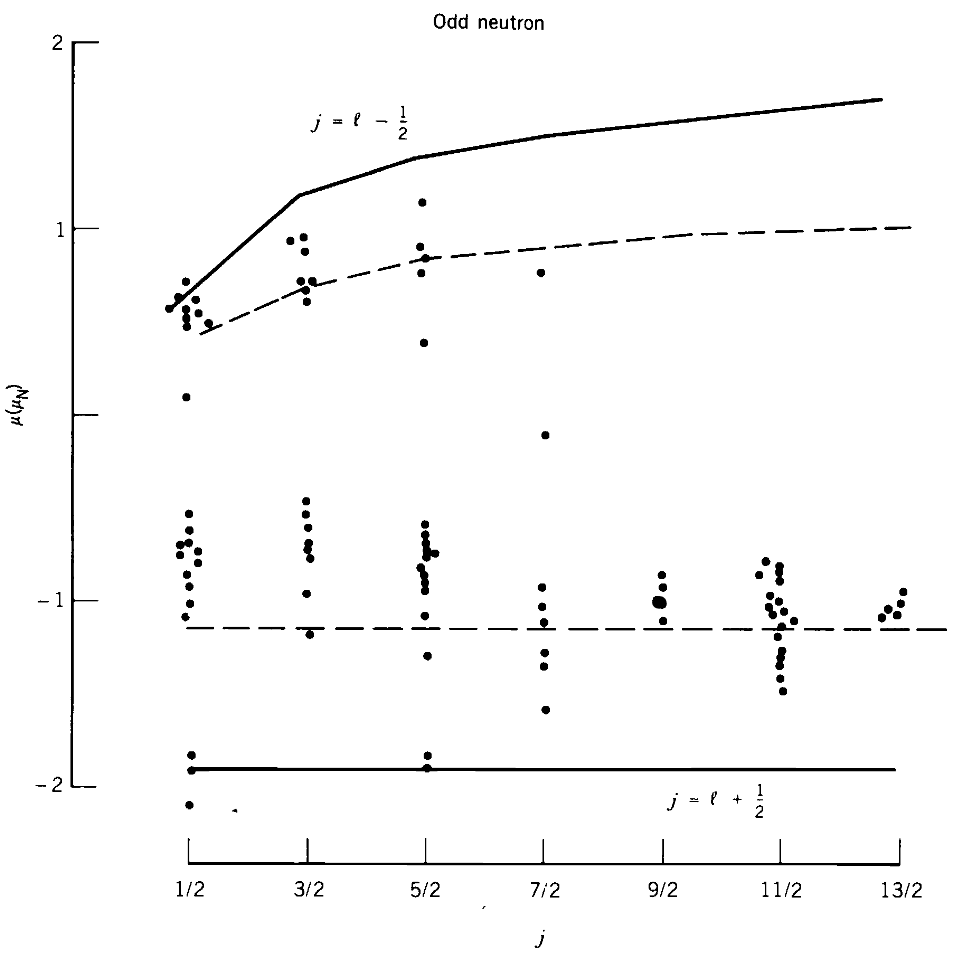
\includegraphics[width=0.60\textwidth]{schmidt-1.png}
	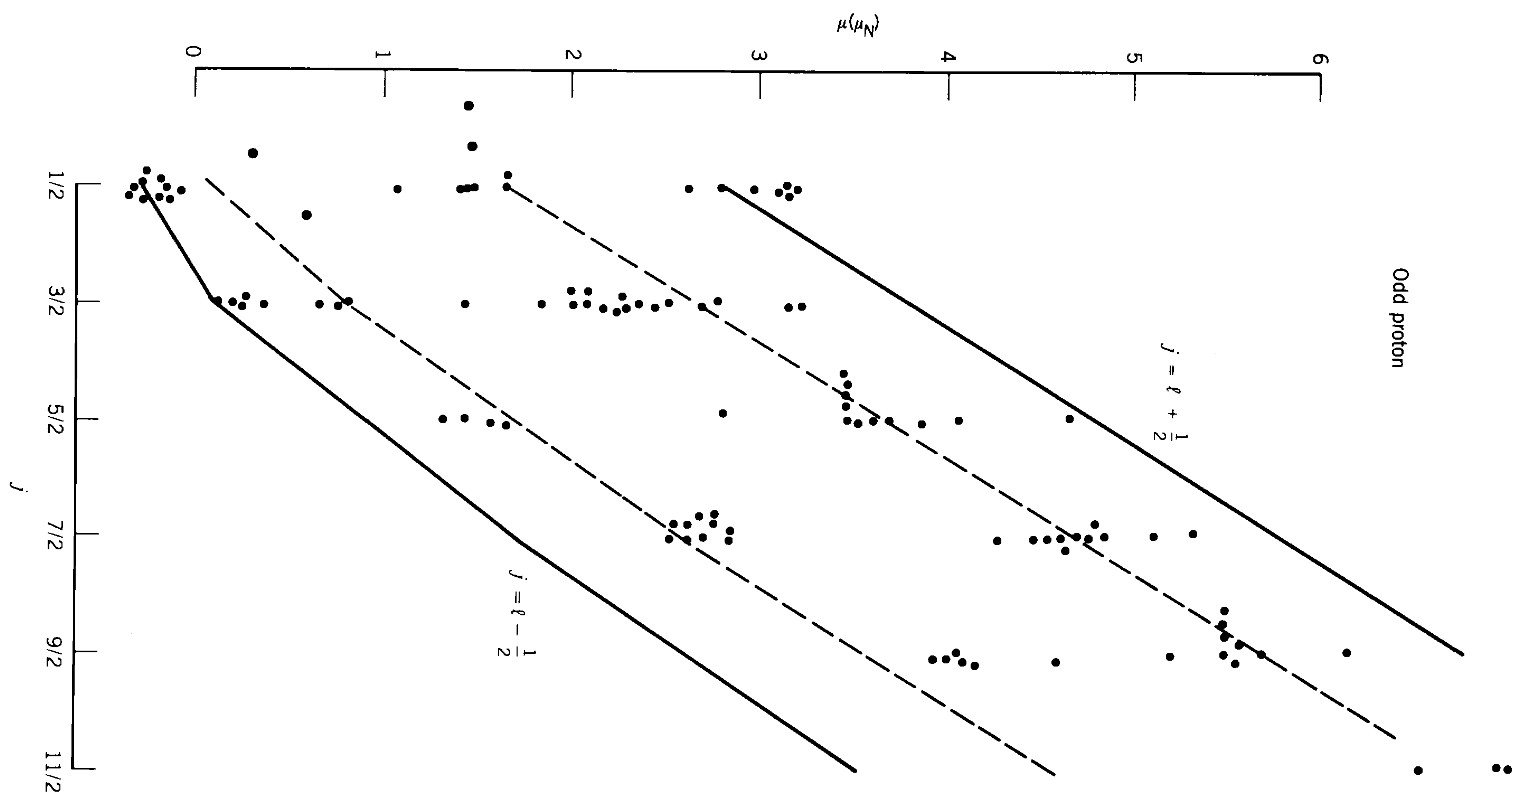
\includegraphics[angle=90,width=0.35\textwidth]{schmidt-2.png}
	\caption{Schmidt lines.}
	\label{schmidt}
\end{figure}

Lo scatter dei dati rispetto alle linee di Schmidt indica che il calcolo del momento magnetico considerando i nucleoni come indipendenti è una semplificazione eccessiva; per un calcolo più preciso, si dovrebbero considerare degli effetti non-banali come l'influenza reciproca dei nucleoni, il fatto che lo spin pairing non sia perfetto, le nubi mesoniche che circondano i nucleoni (che contengono pioni $ \pi^{\pm} $ carichi) e la non sfericità dei nuclei.

\subsubsection{Interazione residua}

Per dare una descrizione unificata di tutti i nuclidi, è necessario aggiungere allo shell model la descrizione dell'interazione residua che viene ignorata nel modello. Ad esempio, per nuclei leggeri è necessario considerare interazioni nucleari a tre o più corpi, problemi difficoltosi da trattare in QCD.\\
Ad oggi, un modo computazionalmente efficiente di calcolare l'interazione residua è dividere il nuclide in un core composto dal più vicino doubly-magic nuclei ($ \ch{^4He} $, $ \ch{^{16}O} $, $ \ch{^{40}Ca} $, $ \ch{^{132}Sn} $ e $ \ch{^{208}Pb} $), il quale rimane freezato e non viene considerato nelle interazioni, e le rimanenti shell d'interazione. Dato che il numero di modi di distribuire $ k $ nucleoni su $ n $ orbitali è pari a $ \binom{n}{k} $, che aumenta fattorialmente all'aumentare dei nucleoni, per snellire ulteriormente il calcolo dal punto di vista computazionale si può ulterioremente restringere l'insieme dei nucleoni sui quali calcolare l'interazione residua alla sola shell di valenza.\\
Anche in questo caso ci sono però delle limitazioni, prime su tutti il considerare solo i nucleoni di valenza e l'ignorare completamente le eccitazioni del core.\\
I principali filoni di ricerca a livello computazionale riguardano da un lato la risoluzione numerica della many-body hamiltonian, dall'altro lo studio delle interazioni nucleari.










